% !TeX root = ../../master_thesis.tex

\chapter{Artificial Intelligence in Commercial Banking} \label{ch:ml_ai}

%\section*{Introduction}
Most of the work in banking industry, which is not connected to human interaction, is over-documented and formalized. 
Having sufficient amount of input data and knowing what kind of output is required it is possible to create a formalized determined way of how to obtain output from input. 
This determined formalized way is called an algorithm.

Main problem of common algorithms is, as it comes of definition, is that it is impossible for an algorithm to solve problems, for which it is not designed.

Nevertheless, it is possible to create an algorithm, that can adapt to changing environment based on previous results.
To find out how to use collect, process and analyze existing data of previous states of environment and corresponding result we can use various statistical instruments.
Aside general statistics, of course, one is able to use tools of data science and machine learning.

As a result, it is possible to create a system, which would be able taking into account primary input data and its own past output data produce new adapted output data corresponding to ever-changing environment.
Thus, having a system which is able to serve decisions, which were not available or known before, we can call this system intelligent.
As a result, we could tell that we had an Artificial Intelligence — AI.
According to European Parliament, Artificial Intelligence refer to systems that display intelligent behavior by analyzing their environment and taking action with some degree of autonomy in order to achieve specific goals.
\cite{ai_ep_definition}
AI is typically defined as the ability of a machine to perform cognitive functions we associate with human minds, such as perceiving, reasoning, learning, and problem-solving. 
Examples of technologies that enable AI to solve business problems are robotics and autonomous vehicles, computer vision, language, virtual agents, and machine learning.
\cite{executive_guide_to_ai}


% !TeX root = ../../master_thesis.tex

\section{Historical aspect of Artificial Intelligence}

\subsection{Decision Support Systems} 

One of the earliest versions of computer intelligence implementations were Decision Support Systems.
Decision Support Systems are interactive, computer-based systems that aid users in judgment and choice activities.
They provide data storage and retrieval, but enhance the traditional information access and retrieval functions with support for model building and model-based reasoning.
They support framing, modeling, and problem-solving.
Decision support systems are typically used for strategic and tactical decisions faced by upper-level management—decisions with a reasonably low frequency and high potential consequences—in which the time taken for thinking through and modeling the problem pays off generously in the long run.
\cite{decision_support_systems_article}

There are three fundamental components of Decision Support Systems: database management system — DBMS, model-base management system — MBMS, and dialog generation and management system — DGMS.
\cite{decision_support_systems_engineering}

A DBMS serves as a data bank for the Decision Support System. 
It stores large quantities of data that are relevant to the class of problems for which the DSS has been designed and provides logical data structures (as opposed to the physical data structures) with which the users interact. 
A DBMS separates the users from the physical aspects of the database structure and processing. 
It should also be capable of informing the user of the types of data that are available and how to gain access to them.

The role of MBMS is analogous to that of a DBMS. 
Its primary function is providing independence between specific models that are used in a DSS from the applications that use them. 
The purpose of an MBMS is to transform data from the DBMS into information that is useful in decision-making. 
Because many problems that the user of a DSS will cope with may be unstructured, the MBMS should also be capable of assisting the user in model building.

The main product of an interaction with a DSS is insight. 
Because their users are often managers who are not computer trained, DSSs need to be equipped with intuitive and easy-to-use interfaces. 
These interfaces aid in model building, but also in interaction with the model, such as gaining insight and recommendations from it.
The primary responsibility of a DGMS is to enhance the ability of the system user to use and benefit from the DSS. 
In the remainder of this entry, we use the broader term user interface rather than DGMS.

First attempts to create and use AI in Decision Support Systems by banks had started in 60s-70s.
Back then, it sounded as something definitely impossible.
Unfortunately, existing state of science wasn't able to satisfy banks' needs and first experience of AI implementation was done only a few decades later.
The pioneer of implementation of Artificial Intelligence System was Citibank.
Specialists of this company made an attempt to implement an automatic Decision Support System that could be as effective, as human experts and more cost-effective.
Generally, Citibank had gotten positive summary.
\cite{decision_support_systems_book}

As a result, leading banks in the United States tried to apply and implement AI as their business solution.
However, due to, comparing with present, low level of development of information technologies, banks found application of AI economically unjustified.
Banks did not invest in continuing researches and for the couple of decades forgot about AI.



\subsection{Contemporary history}

Historically, banks became large financial entities with lots of regulations over them.
This requires from banks humongous levels of responsibility and accountability.
Consequently, banks are known as owners of enormous amount of data, which may be required by regulators, as well as by clients.
Nevertheless, banks are highly interested in using those amount of data for business purposes.
However, both collecting, maintaining, processing input data and using output results is not a simple set of operation.
Having mainly numerical data in digital form, this set of operation requires significant work in terms of Mathematics, Statistics and Computer Science.
This becomes extremely complicated due to previously mentioned gigantic amounts of data, which can easily overpass 1 Terabyte of data a day.

Therefore, that was not a surprise, that Commercial Banking was always keeping its eye on evolution of related technologies.

Even though, banks were using synergy of Mathematics, Statistics and Computer Science since 1950s with varied success, the latest big forward jump was in early 2010s. 

By then, ability to accumulate and process large amounts of data became essential for multiple industries, not only the one, that historically accumulate data. 
\cite{forbes_big_data_history}
Those large amounts of data are usually referred to as Big Data.
Big Data are information assets characterized by such a High Volume, Velocity and Variety to require specific Technology and Analytical Methods for its transformation into Value.
\cite{what_is_big_data}

Since early 2010s, consumer banks started adoption of fast growing Big Data technologies. 
Banks, historical owners of enormous amounts of data, were extremely interested in Big Data solutions and specialists. 
Even though Big Data solves problems regarding collection, maintenance and preprocessing of data, additional tools are required for general processing, data usage and application.
Those tools are provided by Machine Learning.

Most recent advances in AI have been achieved by applying machine learning to very large data sets. 
Machine Learning algorithms detect patterns and learn how to make predictions and recommendations by processing data and experiences, rather than by receiving explicit programming instruction. 
The algorithms also adapt in response to new data and experiences to improve efficacy over time. 
\cite{executive_guide_to_ai}

Obviously, even after decades of research and development those technologies had been still considered as a bit risky.
Therefore, banks had decided to start with something, that would allow reducing costs or optimizing non-operational activity.

On June 2016, agency Reuters issued an article\cite{reuters_ai_hiring}, in which it mentioned that banks of Wall Street in order to try to decrease costs were looking into software development, so it could help to optimize and to speed up the process of searching suitable employees.
For highest performance and due to unpredictable results, banks had bet on Artificial Intelligence.
AI technologies would allow discovering and identify in applicants such qualities, that would be proficient for employer, including ability to works in a team, with a big purpose, willpower, and other soft skills, that,  probably, wouldn't be mentioned in CV or could be found out during interview process.
Hires of bad candidates can cost a lot for a company and lead to large financial expenses and influences negatively for company's business possibilities.
According to experts of Capital One Financial, those losses in average are three salaries of a person, who could fit perfectly for this job.
In such cases self-developing algorithms may allow its clients to get rid of such human errors, as screening out strong candidates, that may look weak at once.
The possibility of implantation of AI to a common process is being under consideration by such financial giants as Goldman Sachs Group, Morgan Stanley, Citigroup and UBS Group.
UBS Group had started using algorithms, that allows to analyze CVs and to find tough candidates as well.
Goldman Sachs Group had used its own software to find specific qualities in CVs, for example, teamwork, honesty and judiciousness.
Furthermore, it uses personality tests for better understanding of qualities of successful bankers and traders.
Some banks used third-party solutions.
For example, Citigroup in June 2016 started testing technology, developed by third-party, to dropout candidates.
Software had been tested on a small group of employees, who had been working in corporate and investment departments.
The application determines, so called, “corporate imprint” — certain set of qualities of existing employees,
which should lead to high corporate performance — and evaluates qualities of candidate based on 
small video, on which job seekers are talking about their strengths and aspirations in career.
That system takes into account not only specific features of job seeker's speech, but also one's skill to present his speech, including body language and rate of speech.
Previously, technologies allowed and helped to find out the best CV, while nowadays it allows understanding people, that apply for a job.
Such solutions give a possibility to drastically remove expenses for unsuccessful hiring and improve the situation on labor market.
In general, Artificial Intelligence allow selecting candidates, that will be able to execute needed work, as it can create templates, based on analysis of big volumes of data.

It may seem, that the changes affected only European and US banks, but AI became a main trend on Asian markets as well.
In Japan, by the end of 2017, it became known about the plans of leading Japanese banks to automate about 30 thousand workplaces until 2027.
Bank boards reached a conclusion, that automatization is inevitable, due to the fact, that traditional methods of making business would not help in increasing incomes.
It would allow minimizing costs of labor capital and direct it to fields, where human workforce would be more valuable.

Those banks assumed, that existing, traditional, business model didn't allow increasing financial gains.
Leading Japanese banks and financial companies, Mizuho Financial Group, Sumitomo Mitsui Financial Group and Bank of Tokyo-Mitsubishi UFJ, informed about readiness to automate more than 30 thousand working places. 
\cite{nikkei_30000_jobs}

According to Nikkei, Mizuho Financial Group are going to replace around 8 thousand employees with computers and increase that number up to 19 thousand.
Sumitomo Mitsui Financial Group started moving towards large-scale automation.
Based on their plans, they were expecting to automate around 4 thousand workplaces by the end of 2020.
Group considered consolidating various clerical work to minimize amount of staff with duplicating duties.
Moreover, around 100 generic routine work tasks would be done by new robotized processing system, that previously had been used by Mizuho Financial Group only for data inputting on opening new investment accounts on its website.
What is even more important, large-scale digitalization did not imply layoffs.
For example, Sumitomo Mitsui Financial Group started its transformation by transferring around 200 back office employees to customer service departments.
Besides, Mizuho Financial Group intends to increase the number of financial technology specialists.
Mitsubishi UFJ keeps up with competitors and plans to automate 9500 jobs up to FY 2023. \cite{mufj_digital_strategy}


Nowadays, the largest market, that uses AI as a solution in the banking sector, remains North America.

In June 2018 Bank of America announced start of research process of using of Machine Learning or currency strategies analysis.
Announced reason for the research was the unstable political situation in Italy — experts feared that it would have a negative influence both on Euro and other European currencies, and this threatens to create new financial crisis.
In the first research Bank of America algorithms of Machine Learning were evaluated by performance of working with fundamental and review data, that involve, for example, governmental costs and expectation of consumer.
The main task of an AI is to create a forecast of relationships of euro and dollar pair.
Due to the nature of the foreign exchange market, it’s rather difficult to forecast using only known situations, and as a result Machine Learning may allow identifying unexpected existing unknown patterns.
\cite{bank_of_america_ai}

As other banks, Wells Fargo \& Company applied Artificial Intelligence in Front Office for customer experience and in Middle Office, for anti-money laundering.
Nevertheless, Wells Fargo \& Company declared that it additionally adheres to a fundamental economic approaches for analysis of foreign exchange markets, as it trusts its experience in this field.
\cite{wells_fargo_ai}

As an example, commercial bank Morgan Stanley hired Michael Kearns, professor of Applied Informatics in Pennsylania University, who had been working in a hedge fund previously, in order to expand the use of AI, while research team of Deutsche Bank had started using Machine Learning for its data analysis.

On the other side, some players did not want to take a risk.
JP Morgan Financial Holdings Research Group had been studying applications for Machine Learning for a long time, but had not decided to use it until year 2021.
Only in first half of 2021 JP Morgan hired 50 artificial intelligence experts and plans to hire at least 160 more professionals.
\cite{jp_morgan_ai}

The fact, that banks are more actively using Artificial Intelligence in applied work was confirmed by Deloitte.
Based on Deloitte research, 
29\% of financial companies, working in different countries, automate most of monotonic routine processes,
25\% respondents use such technologies for risk management,
21\% — for generating risk reports, 
20\% — for regulatory reporting.
\cite{deloitte_thriving_in_ai_era}


The Financial Times made special survey for 30 largest banks, which confirmed a close interest and an understanding of resulting impact 
of swift implementation of modern operation technologies.
Among 18 banks, 17 do already use Artificial Intelligence in clients communication, as it is on this site that they see the most obvious benefits.
8 banks use AI in all structural divisions in any form.
5 expecting in future to have special divisions, which will focus on AI.
8 involved in joint development with specialized companies. 
Moreover, 4 of those even invested into companies, which are exploring AI.
\cite{ai_reality_hype}


Big data and data analysis are still prioritized for banks, as 40\% of respondents use it in everyday data processing.
Around 25\% of respondents declared usage of Machine Learning and 19\% of Cognitive Analytics, including Natural Language Processing, in order to decrease costs and increase operational accuracy, while 24\% of asked banks use it for Business Intelligence.



All over the world, in general in 2018 banks income due to application of Artificial Intelligence was around \$41.1 billion. 
It is important to note, that this amount contains both direct income from implementation of AI technologies, but also
an amount of decreased costs and benefits due to increased work effectiveness of various financial structures, comparing with work effectiveness using same old processes and infrastructures.
And according to market forecasting this income will only grow.
\cite{ihs_markit}

\begin{figure}
    \centering
    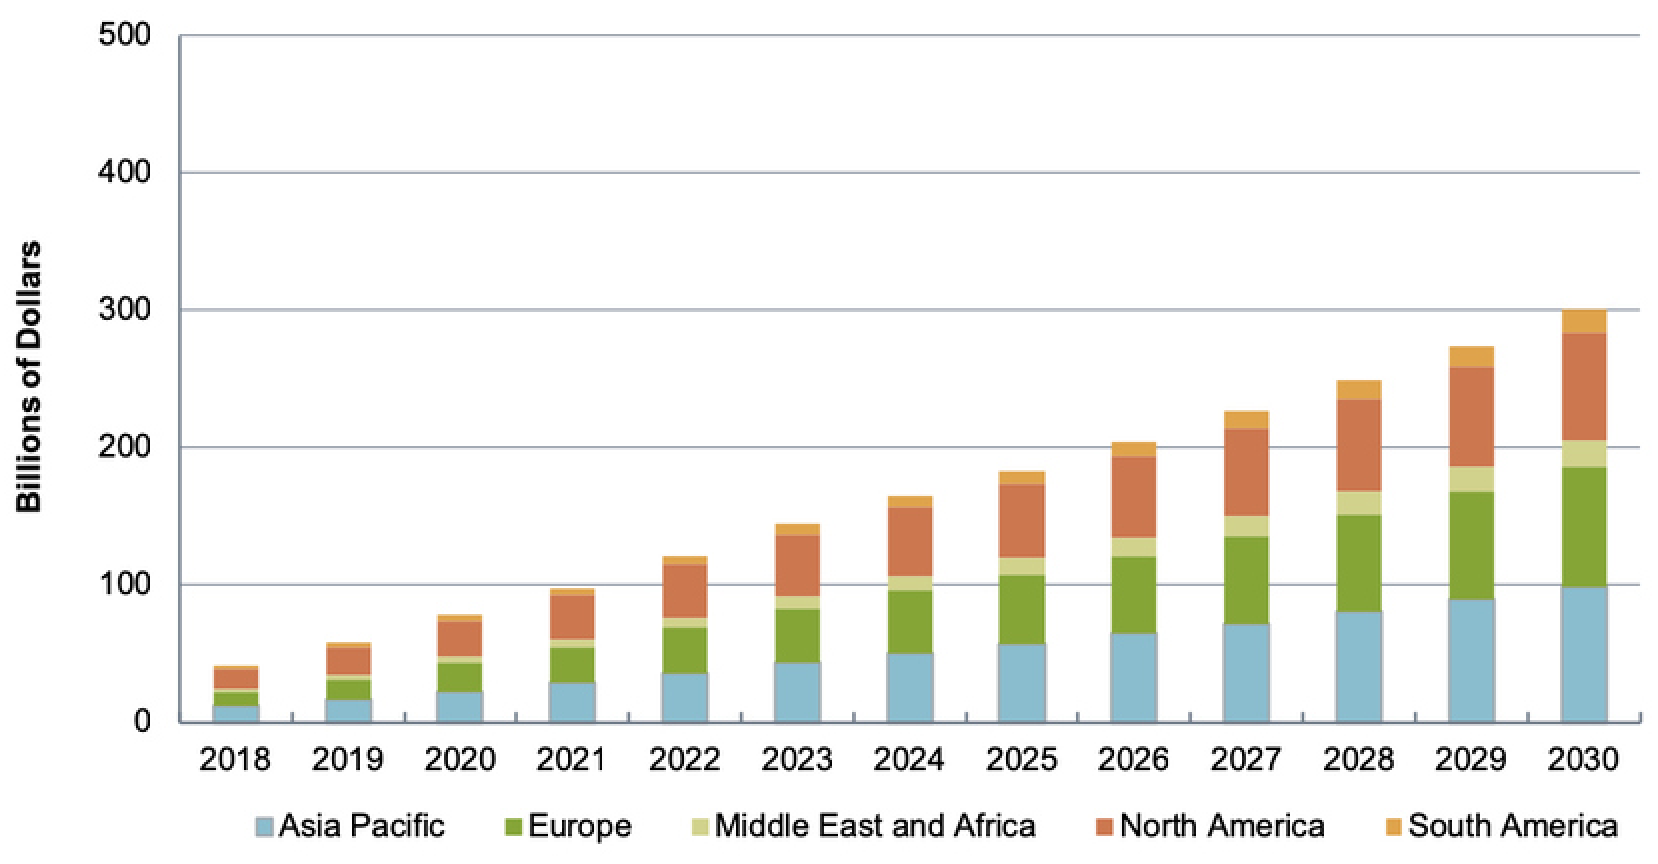
\includegraphics[width=0.8\textwidth,height=\textheight,keepaspectratio]{images/Banking_AI_Business_Value.png}
    \caption{The business value for the world market for AI in banking by region}
    \medskip
    \footnotesize\textit{Source:} "Artificial Intelligence in Banking Report", IHS Markit, 2019, p. 10.
\end{figure}

Even though, as previously mentioned, United States banks are leaders of Artificial Intelligence application, where companies earned additional \$14.7 billion in 2018 thanks to those technologies, experts expect that by 2024 the Asia-Pacific region will break out into the lead, as banks expect to earn and save, thanks to AI, around \$50.6 billion, while in 2018 those banks saved \$11.5 billion.
By 2030 it will raise up to \$98.6 billion due to demand in China (including Hong Kong), Japan, South Korea and Singapore.
\cite{ihs_markit}

According to forecasters, by 2030 banks in the whole world would be able to decrease costs by 22\% using Artificial Intelligence technologies. 
In numbers, this reduction can reach \$1 trillion.
\cite{trillion_opportunity}

According to Accenture, the amount of savings by 2035 will be nearly \$1.2 trillion.
\cite{accenture_ai_banking}

The most tangible changes will occur in units that have direct contact with customers.
By reducing amount of retail divisions, cashiers and security officers, banks cut costs by \$490 billion.
In departments responsible for data processing, analytics and reports, 
introduction of Artificial Intelligence will save up to \$350 billion in middle office and \$200 billion in back office.
In the US banking sector, more than 1.2 million of employees have already encountered AI, even thought they may not be aware of it.


Nevertheless, AI technologies should change structure of financial industry, making bank sector more humane and intelligent.


The profit for the bank is obvious, as it will result in significant cost reduce.
However, forecasts about employment in front banking are much less optimistic.
Recent study of Autonomous Research have shown, that AI can lead to 1.3 million employees losing their jobs in the United States and 500 thousand employees in Great Britain.

Former CEO of Citigroup, Vikram Pandit, who is considered as FinTech evangelist, assume that 30\% of bank employees can be replaced by Artificial Intelligence in near future. 
The threat of layoffs is real for existing bank employees.
Former CEO of Deutsche Bank told, that they intend to replace 98 thousand of workers with smart software solutions, while
Japanase Mizuho Financial Group will free 19 thousand of workplaces, third of entire stuff, by 2027. 
\cite{ai_reality_hype}


IHS Market assumes, that among bank employees, who can lose workplaces, the biggest risk is for B2C front-office workers, especially, cashiers, customer service, interviewers, clerks, financial managers, controllers and credit specialists.
\cite{ihs_markit}


Even though usage of Machine Learning for complex analysis is not an innovation, according to Vasant Dhar, Informatics Professor in New York University and founder of SCT Capital Management Hedge Fund, which has been applying AI for 20 years, foreign exchange markets are still a significant challenge for AI algorithms and modelling.
Complexity and variety of macroeconomic factors, which can have influence on inter-currency relations, crucially complicate analysis for foreign exchange markets, unlike regular stock markets that has been using AI and ML for a long time.

Main criticism of AI is based on lack of trust to results, as ML supposes Black Box analysis and finding interconnections in unpredictable ways. 
Therefore, most of the critics cannot accept prognostic findings to AI, as it processes data without building relationships
between cause and effect.

Despite rational enormous cost savings, a number of researchers are recommending to step off radicalism.
In their opinion, banks should be careful not to rely too much on new solutions.
Its effectiveness is extremely clear only in case of complementing human work, not replacing.
Therefore, introducing artificial intelligence, banks should be prepared at least to educate employees of robotized work process.
Large Dutch bank ING agrees with this position:
“We would like to use artificial intelligence in order to suggest more thoughtful decisions to our clients and to be more effective in decision-making, and not to replace workforce with AI”.
\cite{ai_reality_hype}


On this direction there is a temptation to improve the artificial intelligence, making its possibilities closer to human ones. 
Unfortunately, much still remains outside the perimeter of capabilities of modern technologies.
AI has a function of recognition, but not of cognition. 
It is wrong to assume that humans and machines can work on a same level.
It would be a long way, and it would require significant research until machines begin to at least approaching level of human performance.
Predictions regarding the timing of the creation of truly “smart” intellect are pretty vague.
\cite{ai_reality_hype}


Doubts arise not only in terms of timing.
Considerably more important are considerations of a generalized and even philosophical nature, for example, whether it is generally necessary to strive to model human thinking in its entirety.
The spheres of application of human and machine intelligence should coexist in complementarity, and not repression (or replacement)
In a number of situations, there are no simple tasks that can be solved purely algorithmically, but a human mind is needed to cope with them.
However, humanizing artificial intelligence deprives it of those strengths, for which, actually, human tries to create and swap himself with rational, algorithmic and objective source of actions and decisions.

Digital economics brings changes not only to operational bank activities, but also into relationships within community of financial institutions.

Research conducted by World Economic Forum together with Deloitte and Touché led to the conclusion that possibilities, which are being brought by Artificial Intelligence are an option only for the largest banks.
Since the main innovation concentrate on customer acquisition channels, then it is very likely to observe banking sector regroup — the dominance of large structures and the withdrawal from the market of small and medium structures.
\cite{ai_transform_disrupt}

However, researchers leave small companies a chance on survival.
Those assume that smaller companies have an option to specialize in certain directions, types of operations and specific clients.
Consequently, along with large banks, customer service in digital economics may be provided by small niche financial companies.
\cite{banking_ai_revolution}

The desire of benefit by expending of information base and Artificial Intelligence, which is the main data consumer, will lead to creation of monopolies — large alliances of financial groups.
The need of strengthening and enhancement of bank cooperation is required by increasing importance of analytical work, grow of risks of cyber-attacks and fraudulent schemes. 
The effectiveness of protection against criminals significantly increases in the conditions of sharing information about criminal patterns, sharing blacklists of companies and clients.

Nonetheless, transfer, control and usage of received data has to be settled down, including legal establishment.
Data owners, as well as clients, are interested in reliable control over data.
As a result, there is a need in obvious legal procedure of personal data transfer and its protection.
The transfer of activities to digital space creates entirely new risks and requires new methods of risk countering, which have not been worked out yet.

At the group level banks agree on a fact, that main route of development of banking is based on implementation of opportunities offered by digital economics.
Moreover, banks apply the latest achievements of computer technologies and software development, among them Artificial Intelligence, in individual areas of its work, replacing an employee with robot on routine repeating operations.
Nevertheless, banks are very careful about complete and deep technical restructuring, sending significant funds for studying the issue.
Regarding modern stage of Artificial Intelligence application and immediate prospects, I would like to cite The Financial Times:
8 years ago there was a talking robot in Santander Citi, but none of them is left in any of 13697 branches of the bank.
\cite{ai_reality_hype}

Even nowadays, banks are still focused on creating necessary conditions for AI transformations, including preparation of infrastructure, data, models and processes.
In addition to fields, that always have to be on the cutting edge, in order to gain advantage as a pioneer, 
changes are coming to more conservative spheres of financial services.
Despite the active usage of Artificial Intelligence, most banks have not had time to implement it globally yet.
According to experts, overwhelming majority of financial institutions noted usage of Machine Learning in one degree or another, but, as it had been noted by experts, only 20\% of respondents went beyond the basics of AI usage.
\cite{ai_reality_hype}

But structurally, banks were creating single open platforms, which provide general service for all domestic business customers.
Therefore, there is a need in relevant professionals, who would be able to handle and support platforms.

% !TeX root = ../../master_thesis.tex


\section{Artificial Intelligence in Operational bank activity}

Nowadays, banks are equipped with modern information and communication technologies.
At the same time mentioned technologies, including Fin-Tech software, have significant impact over existing financial institutions.
By surpassing operational limitations, those technologies become the main factor of transformation of both in a case of single bank, and in a case of entire banking sector. 
This results in a gradual increase of computerization of banking industry, leading to larger possibilities of application of artificial intelligence.

Significant volumes of information are being accumulated over financial markets resulting in data analysis being more and more relevant.
Some experts note, that markets are already emerging where data sharing is critical to competitive success and first movers are positioned to distinguish themselves by delivering better advice, constant presence, and curated ecosystems. 
Firms that lag behind are finding that their old strengths may not keep them as competitive as they once were.
\cite{ai_transform_disrupt}


\subsection{Artificial Intelligence in Investment Banking}

The pioneers of application of modern Artificial Intelligence and related technologies are, obviously, investment banking companies, which had to apply modern solutions in day trading algorithms. 
Those companies target Machine Learning and Natural Language Processing in order to use it for data, news and content analysis.
For them the most popular source of alternative data are news aggregators, expert networks and search query indexers.

Most of the asset managers and hedge funds specialists suppose that according to existing competitive dynamics, the trend of research disaggregation will continue even in regions not covered by MiFID II, legislative framework instituted by the European Union to regulate financial markets.

There is a popular opinion, that during researches investors would rely less on investment analysts. 
Some expect major changes in investment research market, as investors would need more data for support of AI and Machine Learning technologies.
On conducting researches, portfolio managers would rely less on investment analysts and more on internal solutions, data suppliers and solutions suppliers.
\cite{future_of_trading_technology_2024}


\subsection{Artificial Intelligence in Commercial Banking}

As for commercial banking, the status of AI integration highly depends on bank size.
All over the globe major financial players have been developing solutions based on Artificial Intelligence for the last 60 years with the various levels of success.
The situation has been especially progressive for the last 10 years.
In general, over 70\% of large global banks studied and have implemented AI for front-office or back-office functions.
\cite{deloitte_thriving_in_ai_era}

However, as for middle-size financial institutions, situation seems pessimistic.
While largest banks have been developing AI strategies, creating teams and projects in place by investing billions of dollars, for midsize banks AI was not even on the radar.

In comparison, while large banks have been investing majorly since 2016, in 2020 less than 20\% of midsize, or less, financial institutions invested in, implemented, or at least planned to apply AI.
What is even worse, only 2\% of those have deployed chat-bots, Machine Learning or other Artificial Intelligence technologies.
\cite{ai_transform_disrupt}

The main reason is in AI capital limitations.
Even though, those technologies can be independent of existing business structure, the last are highly dependent of capital investments.
Therefore, large financial institutions Banks that act now can capitalize on the power of automation and intelligence to truly transform their organizations.


Midsize and smaller banks and financial institutions have to compete with mega-sized counterparts without R\&D budgets.
What is even worse, the gap between large and non-large institutions only increase, because of how AI works.
The longer AI operates, the smarter and more useful it becomes.
As a result, the longer financial institutions wait, the harder it becomes to catch up. 
Financial institutions that start early gain a head start of months—even years—to gather data and “train” their self-learning, intelligent applications. 


Consequently, currently Artificial Technologies are available mostly to big players.

However, for midsize and smaller institutions not everything is lost, as there is a third-party option.
Machine Learning and Artificial Intelligence is highly used in start-ups, and application of solutions of those may save capital for research and development, and would allow applying tested solutions.
Secondly, most AI start-ups are small. 
Pilot programs and third-party innovation labs give banks and credit unions a chance to test, learn and refine your AI initiatives for a relatively small cost, before seeking funding for full-scale roll-outs.


However, one of the most important question of this analysis is what should banking acknowledge as Artificial Intelligence, what are its forms and possible use-cases in practice.

Currently, there is an extremely wide range of opinions.
Due to lack of unified theoretical platform of banking services, forecasts of development of banking institutions based on AI differ drastically and are based on business strategies of every single bank.
Nevertheless, there are 2 main routes of development.
First route is about focusing on cost reduction by workforce replacement and automatization of repeating routine operations without significant reformations of existing organizational structure.

On the other hand, there is a perspective in new digital technologies, which may allow inventing and introduce qualitatively different business models based on new market challenges, and, as a result, developing brand-new sources of income.
\cite{ai_reality_hype}

Nevertheless, in general, Artificial Intelligence in banks can be used in lots of areas.
From bank's perspective AI is needed from its ability to harness bank data in three key ways: to analyze, to act, and to improve by self-learning.

Systems of Artificial Intelligence were developed for automation of clerical workload, other routine paperwork, processing of various data sets.
In the digital age, banking transaction operations are just a form of abstraction over data transfer and storage.
Even though largest banks prefer to save more traditional organizational structure, they actively embed digital technologies in everyday practice.
Even though, banks prefer a less risky way, Artificial Intelligence application is applied in all bank fields, on all office levels and has to be precisely analyzed on each of those levels.



\subsection{AI in Back office}

Both Artificial Intelligence and Machine Learning may have significant influence on entire Back Office of Commercial banking.
Back office is known for enormous amount of repeating actions due to Execution, Clearing and Settlement process.
Therefore, the primary appliance of AI is in automatization of repeating routine operations.
Automated solutions, that automatically builds behavior patterns is ideal of Back Office, as it initiates high back-office efficiency via automation.

Ironically, this case is the case, when human intervention can impact more negatively, than positively.
For repeating actions, for example, calculations, in which there is no responsible decision-making, artificial intelligence suits the most.
“For repetitive tasks without variability (in middle office, in back end) for clearing/settlement/operational processes that are not particularly in need of smarts, 
then AI approaches are great,” says Pascal Bouvier, a venture partner at Santander InnoVentures, a fintech venture capital fund of the Spanish bank that invests in early stage Fin-Techs including those focused on AI.
\cite{ai_reality_hype}


Special attention of applied automatization is directed into processes, that require large amount of work, but offer low profitability.
McKinsey shows as an example of JP Morgan, which had started using chat-bots for IT service request automatization.
In 2017 1.7 million of requests where processed this way, which is equal to yearly full-time workforce of 40 employees.
\cite{ways_ai_transforming_bi}


In fact, it is possible for bank to transfer to robotic solutions such operations as:
\begin{itemize}[noitemsep]
    \item Payments processing of legal entities and individuals
    \item Processing of unidentified payments
    \item Customer data change based on statement
    \item Editing credit agreements based on individual statements
    \item Document processing
    \item Credit underwriting
\end{itemize}

Another popular application is processing of incoming documents.
Modern scanning programs can recognize standard documents and transfer them to performers.
Naturally, this kind of programs contain special filters, which direct documents, that do not fit into specific characteristics, for expert review.
Moreover, modern systems allow recognizing most typical types of documents and fill it using typical forms.
This allows a practical usage of these tools for legal office and even compliance control divisions.
As a result, activity of institutions become aligned to established regulations.
However, undeniable benefits of automatization based on artificial intelligence can be fully achieved and felt only in case of continuous update and upgrade of technological base.
\cite{banking_ai_revolution}

As an example of direct application, it is possible to refer to remittance matching solutions, that improve straight-through processing.
As an example, Deluxe offers AI based payment to remittance matching, which should shorten Days Sales Outstanding resulting in a same-day posting
\cite{deluxe_ai_remittance}

% if more needed: https://internationalbanker.com/finance/artificial-intelligence-storms-back-office/


\subsection{AI in Middle office}

In comparison to Back Office, where AI may be used primarly for infrastuctural changes and evolution, Middle office is open for the biggest cost cuts and optimizations.
According to researches, Middle Office alone can save \$217 billion, around 50\% of all cost savings available by AI for banks by 2023.
\cite{trillion_opportunity}

The reason for this is hidden in a definition of Middle office by itself.
Middle office is comparably new division of a commercial bank, and usually forms a bridge between customer flexible Front and strict and executive Back office.
Hence, Middle office operations by its nature are structured and documented, but have a certain level of statistical disturbance.
Thus, it makes Middle-office the most interesting and sensible target for AI development for commercial banking.

Importance is based on a combination of possible backfire of operation logic and unpredicatable patterns, that can form in everyday work.
This leads to, probably, the most obvious area for AI in Middle office — Credit Scoring.
AI in this case allows calculating credit scores not only based on known mathematical models, but to find out new, previously unknown patterns.
As an example, credit risks for private clients can be analyzed based on user's digital footprint, that can reach enormous amount of data.
Moreover, this may be true for clients, who have no credit history, or very old credit history, as it would allow to set a credit score based on a data of other clients.

Secondly, AI has a major usage in Anti-fraud.
Practically, it has the same reason to use as for Credit Scoring — it is possible to unite existing models with unpredictable patterns.
In this case model can analyze not just payment data, transaction history, transaction time and location, but in a various combinations based on possible patterns of transactions of other users.
Additionally, AI supports and provides face recognition systems.
As for ATMs, all actions can be guaranteed by face recognition.
It is true for Internet Banking for customers and CRM for bank employees as well.

Furthermore, the same reasoning is true for both KYC and AML compliance.
In general, Artificial Intellegence brings multiple possibilities for KYC and AML, such as unified pool of data, probabilistic matching, progressive evolution, self-training and pattern-based analytics in conjunction with rule-based.
Moreover, these features allow using AI in Risk Management, for credit and risk underwriting.

% proof: https://www.h2o.ai/resources/solution-brief/know-your-customer/

Based on existing estimations, around 20\% of digitalization projects are targeting cost reduction or productivity increase.
Most of those are targeting on potential risks recognition and minimization of risk consequences.
\cite{ai_reality_hype}

Artificial intelligence may frame out unlawful behavior, including non-stereotypical one.
By processing big data artificial intelligence may find out an evidence of fraud or illegally money laundering attempt.
The most simple way, but still significant, criminal pattern identification and revealing unlawful activity.
 
Artificial Intelligence can cover large databases and catch patterns, which hide from human attention.
Even more complicated approach of AI usage is educating to identifying market noises.
As a result, more advanced technologies allow discovering and determine people and companies with elevated risk for banks, allowing to build safer relationships with them in future.

Crimes in virtual banking are evaluated in \$600 billions yearly.
Artificial Intelligence and Machine Learning as main instruments for risk management in banking practice are mainly oriented on financial crime prevention.
This is much more efficient, comparing to complicated processes of damage compensation and financial crime evidence confirmation search.
Mastercard, for example, was able to reduce attacks on customer accounts by 80\%.
\cite{ways_ai_transforming_bi}
 


\subsection{AI in Front office}
\label{subsec:ai_front_office}

Numerous Financial Instituations are leveraging AI-driven chatbots and algorithms to support existing customer service channels with faster, more consistent intelligence.
One of the common thoughts on AI application in Front office are Biometrics.
Biometrics are widely represented by various recognition systems for much safer authentication.
Voice recognition is used to determine client by voice, facial recognition technologies, which are based on ML and AI, help to determine a client or to check correctness of client's photo data.
Similarly, Computer Vision technologies allows to determine the authenticity of physical signature.
However, it is more correct to consider biometrics as an input for Anti-fraud systems. 

As a minor use case, Front Office is interested in offering Personalized financial products, but this solution can be interesting for financial aggregators and Banks-as-a-Platform, but both those forms of financial institutions are comparably immature.

Even more rare is an application of AI in case of Robotic Advisors and Algorithmic trading on a consumer level.
However, it became more active since last year.

This is an alternative to communication with financial consultants in order to create and manage investment portfolios
with stocks, bonds and other assets.

In just a few minutes, according to the set parameters, the robot advisor can assemble a balanced, by industry and company, investment portfolio, taking into account the available investment amounts, with the optimal ratio of risk and profitability.

It is believed, that those systems can create accurate forecasts for stock market environment, due to possibilities of
automatic collection and analysis of the state of foreign exchange markets and latest economic news.
This allows client to invest into tools with the lowest risk.

Robo-advising became a powerful alternative to financial consultants in basic questions, related to banking, financial management and cash transactions.
The portfolio in the US financial markets, which is now being managed by robots, have already reached \$1 trillion in 2020
and rapidly increases, expecting to make up its volume up to \$2.85 trillion in 2025.
\cite{europarl_roboadvisors}

Going further, AI can be widely used not only for helping clients with investments, but in entire Individual Banking.
Standardized financial products and services for wide range of consumers cannot satisfy needs of modern client.
Modern clients require personified conditions for accounts, loans and other services. 
Without individual approach it is impossible to implement, therefore, one would need Artificial Intelligence as well.
Nowadays, every financial entity develops and offers between 10 and 20 financial products.
For developing such products banks need a team of professionals.
Developing hundreds of thousands of personified offers for every bank client is, by fact, impossible without help of Artificial Intelligence.
According to statistics, nearly every person has between 2 and 5 electronic devices, which can connect to internet, use various messengers or social networks.

Naturally, every internet user leaves enormous volume of data after himself.
Analyzing that personified data effectively allows creating various unique personified advices and offers.
Algorithms of Artificial Intelligence, theoretically, can collect client information, analyze and generate individual personified offer.

As a result, whole service industry becomes more and more personal.
Screening social networks profiles, collecting GPS or any other position data allows classifying client and to create his social portrait.
Obviously, from bank's side, it allows to effectively determine credit rating for every client.
At the same time, as an example, if one works in an agricultural field, bank can suggest and recommend various products connected with harvest insurance.
As for small business, analyzing supply chain and contragents of that business, bank can at the same time analyze seasonality of payments and more accurately predict time ranges, during which client liquidity can drastically decrease, or possible cash gaps.
This knowledge allows bank to operate more effectively and saves business from a useless hassle.

At the same time, case of Conversation Banking is extensively developing and has to be precisely analyzed.
Conversation Banking for the last 3 years became extremely popular.
Among the largest U.S. and international banks, the greatest focus today is on conversational interfaces, such as chatbots and virtual assistants.
\cite{deloitte_thriving_in_ai_era}

The main purpose of Conversation Banking is a client communication.
Nowadays, there are general purpose AI programs, that are able to speak to people.
Having a chat-bot call assistant for common problems allows bank to extend it into artificial personal assistant, including financial one, that can help a bank client using his and only his data.

Chatbots are one of the most effective ways to answer questions from employees and customers.
Client can call to a bank and talk about his problem, but due to the fact, that this problem can be categorized, a client can talk to bot, that can help client to solve his problem and tell about some problem related services.
Moreover, it can analyze client needs and immediately provide various financial recommendations.
Of course, that can be presented with any form of communication, both with SMS, internet messages or voice messages and calls.

But there is even more interesting point of view.
Based on the various researches, banks that are targeting teens and younger adults has to take to its concern, that younger people are not used to talk over phone, but to contact via messengers. 
Therefore, banks have to develop text chat-bots, and on various platforms, including bank's website, bank's mobile application, and chat-bots for application, where those people prefer to use, like Facebook.

In addition to chat-bots, banks can use voice assistants.
According to him, the assistant will help users in solving financial and everyday tasks — money transfer or reserving a table in a restaurant.

For example, Apple Siri, Amazon Alexa and Google Assistant are tightly coupled into everyday life of modern people and access to such fields of can result in an extremely high level of interaction between bank and client, and, therefore, increases client's loyalty. 

Bank's client can ask in this case various general questions and receive answers immediately.
For example, client can ask what payments were done with debit card last week, 
level of debt of a credit card and when fixed-term deposit ends.
As a result, client doesn't spend time looking for information on bank's webpage, sorting history in mobile or web app.
The assistant has another area of usage as well. 
For example, using an installed app, that is able to recognize products on store shelves, assistant can display cashback amount, which would be returned to the client after paying by credit card.

As a result, client communication is expected to outlive vitaly crucial challenges. 
Firstly, there is a growing competition over clients, both in attraction of new and in retention of old ones.
Secondly, ready-made technologies may allow to execute this much more effectively and with lower costs, then an operator.
Basically, almost all banks replace communication employees with a program — the chat-bot.
Usually this transformation is being done painlessly for a bank, as in most cases a foundation already exists.
In recent years operators were building client communication based on a script, scenario of a dialog.
In case of more complicated talk, operator have to transfer a talk to a manager with more responsibilities.
Based on research, modern chatting solutions can not be distinguished from an alive person by 60\% clients.
Chat-bots are attractive for business by providing consistent access to bank information with an immediate feedback, which is extremely important for the client.

Response delayed by 5 minutes decreases chances to create long-term bonds with a client by 10 times, resulting in building bonds with a bank, that answered the call, as in this case client feel himself important. 
Nevertheless, it is still important to leave a possibility to contact an alive employee, as 79\% of respondents would positively react on a conversation with a human,
while 74\% negatively react, if they would have a conversation with a machine, without a possibility to have a contact with a human.
However, modern programs may transfer communication to an employee, who has much more possibilities to handle a non-typical talk.
Client is important for a bank in case if he is using bank services on a regular basis, and constant contact is a reason of 70\% of purchases of banking services.
Chatbot, as a universal worker without breaks and competitors, especially for big banks with large client base, which bank has to be in a constant contact with.
Nowadays, such robots to a large extent are replacing call centers, mailing centers and in certain cases marketing divisions.

Swiss bank UBS, which is in Top 50 by assets, developed service Ask UBS to serve companies which specialize over managing client finance.
Offered service allows receiving advices in wide range of questions and financial markets analysis.
Moreover, it works as an educational service, clarifying definitions, giving definitions to acronyms and translating professional slang of the financial market.
According to UBS representative, bank intends to turn Ask UBS into a common instrument, which could be “secure, compliant, and trustable for clients.
\cite{ways_ai_transforming_bi}

Correctly developed program may not just execute multiple routine functions, but have an ability for self-education and self-correction.
Some specialists assume this would not be any burdensome development, if software developers didn't receive overcomplicated requirements.
However, extremely complicated solutions supporting multiple platforms and self-learning may be pretty expensive.
Therefore, most banks start exploring the digital world of chat solutions with simple virtual agents, which is mostly based on scripting and scenarios.

Another important direction of client communication improvement is the personalization of products and services.
Personalization is one of the main, if not the main, instruments for competition in banking sector.
Previous criteria of competitiveness, as price of banking products,  service delivery rate and accessibility, are fading out in significant extent, especially due to the fact of equalizing of competitors due to equivalent access to modern technologies, leaving no place for tangible superiority.

Competition over bank client moves towards digital solutions with the priority to develop client adapted, demand-based product, to form convincing recommendations, up to ready-made solutions, based on client needs, thoughts and expectations.
Banks obtain possibility to influence actively on client behavior by using large amounts of data.
By processing that data, artificial intelligence receive an option to offer client personified product on best suitable user conditions, as it, obviously, considers client's targets and financial possibilities.
It is common for such products to get ahead of client wishes, resulting in forming request by consulting and clarification.
\cite{ai_transform_disrupt}

Santander bank even instituted an award for developing a program, which would allow joining banking products with client needs.
\cite{ways_ai_transforming_bi}
In this part of banking the importance of consultants and intermediaries in relationships between banks and clients is increasing.

Naturally, conditions of digital economics allow for a robot to be the consultant, which would make recommendations about better products, institutions and services oriented on specific client.
This results in a trend of separating it into independent activities without binding to a single financial company.

Possible options of activity for general purpose solutions are much wider, as such solutions are not only based on bank products and services, but those can offer interaction with companies with more favorable conditions.
High level of personification of service and demand for intermediate service providers may even lead to the extintion of traditional forms of product offering, which is currently based on each product separately, for example, debit cards, payment systems, loans and saving accounts.
Instead of traditional offering, digitalization allows for development of universal financial service, which would implement all financial client requirements in a single integrated service, and what is more important, in way which would fit client needs the most.
One more step towards banking automatization is remote customer service for a certain range of operations.
Such possibility can be offered by a solution, identifying client by specific features — facial features, voice features or finger capillary network.

There are even more exotic options. 
For example, one Japanese researcher suggest using individual person's blinking behavior.
British bank Halifax conducts test of a special bracelet, which would register individual heartbeat features.
\cite{ways_ai_transforming_bi}

Some of those technologies have already been tested in production for financial operation. Most known example is the Apple Pay on iPhones, which uses facial recognition not only for phone unlocking, but also for executing operations via Apple Pay and other digital wallets.
Specialists claim that ways of person identification are becoming more complicated. 
On the other hand, those technologies at the same time become much more reliable and stop being exotic.

Google Intelligence predicts that by 2021 1.9 billion of bank clients would use biometric data for remote services.
However, there is still no large demand by banks for such remote forms of service, even though those technologies of identification have been developed long time ago and even tested by bank security services.
This is mainly due to lack of guarantee for operation to be voluntary, without any unlawful influence and there is no satisfying solution for such problem yet.



%\section*{Conclusions}
Artificial Intelligence has already become a leading driver for technology innovations in banking sector.
It has already been developed enough and definitely reliable in everything regarding risks, confidentiality, human factor and marketing strategies.

Nevertheless, AI has already changed financial business and will change it even more in near future.
The vast majority of actions, that are being done both in back-office, middle-office and front-office by employees can be automized and algorithmized.

\begin{table}
    \centering
    \begin{tabular}{| c | c | c | c |}
        \hline 
        \textbf{Divisions} &
            Front office & 
            Middle office & 
            Back office \\ \hline 
       
        \textbf{More mature} & 
            Conversational banking & 
            Anti-fraud, KYC, AML & 
            Credit underwriting \\ \hline 
       
        \textbf{Less mature} & 
            Biometrics & 
            Legal and Compliance &
            Smart contracts \\ \hline 
        \textbf{Savings} &
            \$199 billion &
            \$217 billion &
            \$32 billion \\
        \hline 
    \end{tabular}
    \caption{Fintech AI Use-cases}
    \medskip
    \footnotesize\textit{Source:} Own study, based on: Lex Sokolin, Matt Low, "\#Machine Intelligence \& Augmented Finance", Autonomous Research, p. 29.
\end{table}

The main interest for banks is in application of AI in front-office and middle-office, as it will lead to significant cost reduction, up to \$400 billion in 2025.
Banks use AI in front-office for identification and authentication of clients, in order to imitiate alive workers with chat-bots and voice assistants, to deepen relationships with customer, increase engagement, and to offer personalized ideas and recommendations.
Additionally, AI is being used in middle-office.
It allows detecting and preventing frauds with payments, upgrading processes connected to anti-money laundering processes and detection for know your customer control systems.
Those sources of income, which have already been transformed by AI, show the valid way to use this possibility.
Nevertheless, those strategies show that banks have to create holistic strategy, which would connect and cover multiple scopes of banking, sources of useful data, third-parties and employees.
\cite{autonomous_next}

However, with all the advantages of modern software, forecasts of full robotization probably won't be realized, as in near future it is unlikely for a program to replace a person.
\cite{deluxe_mid_size_banks_risk}

In order to integrate the foregoing into existing banking service it is necessary for banking platform to support it.
Obviously, those platforms, which current banking stands on were developed around 15-30 years ago, or even more, and this makes integration of modern algorithms almost impossible. 
This is why modern banks are now puzzled if it is possible to reengineer their software in order to have an effective possibility to embed Artificial Intelligence and Machine Learning in its banking platform.

Nevertheless, it is extremely important to remember, that automating workplaces doesn't always lead to dismissal of workers.
It is important to create retraining programs, that would allow existing employees to obtain new skills in fields,
that are out of risk of automation, in order to decrease automation's influence on labour market.

Increasing number of internet users, availability of smartphones and other handheld devices, and rapid development of mobile internet forms new users' habits and behaviors.
Social network users and mobile app users are more and more focused on getting instant results and target specific actions with the lowest amount of clicks possible.

However, the need of receiving high-quality financial services and personal consultations hasn't disappeared: people are still calling to call-centers.
Even though remote banking service systems are rapidly developing, number of phone calls recently significantly increased. 

Nevertheless, there are good news for banks that have yet to embark on their AI journey. 
Making progress in AI does not require an unbearable effort.
It typically begins with identifying your organizational goals, readying your data and finding the right partners.
Nonetheless, even medium-sized and small banks have to investigate this topic by now, as in future, gap between AI users and nonuser will only widen.





